\chapter{Tổng quan lý thuyết}
\label{Chapter2}
\section{Mô hình Transformer dịch máy}

\subsection{Tổng quan mô hình}

Transformer là một mô hình có kiến trúc encoder-decoder. Mô hình bao gồm 2 thành phần chính là Encoder(bộ mã hóa) và Decoder(bộ giải mã). Khi đưa một đoạn văn bản nguồn vào, mô hình sẽ xử lý vào đưa ra đoạn văn bản có ngữ nghĩa tương ứng ở ngôn ngữ đích.

\begin{figure}[H]
    \begin{center}
        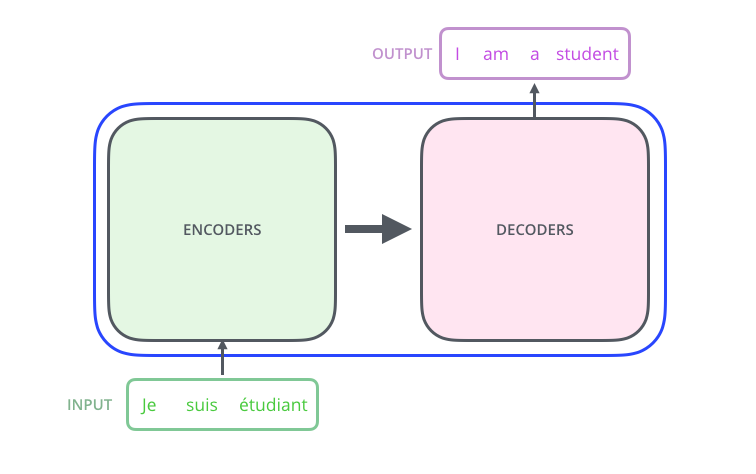
\includegraphics[scale=0.4]{images/The_transformer_encoders_decoders}
        \caption{Encoder-decoder}
        \label{fig:encoder-decoder}
    \end{center}
\end{figure}

Cụ thể hơn, Bộ mã hóa sẽ bao gồm nhiều lớp mã hóa xếp chồng lên nhau. Theo paper transformer, họ sử dụng 6 lớp mã hóa để tạo thành một bộ mã hóa.  Bộ giải mã, tương tự cũng được xếp chồng bởi các lớp giải mã. Số lượng lớp của 2 thành phần phải bằng nhau.

\begin{figure}[H]
    \begin{center}
        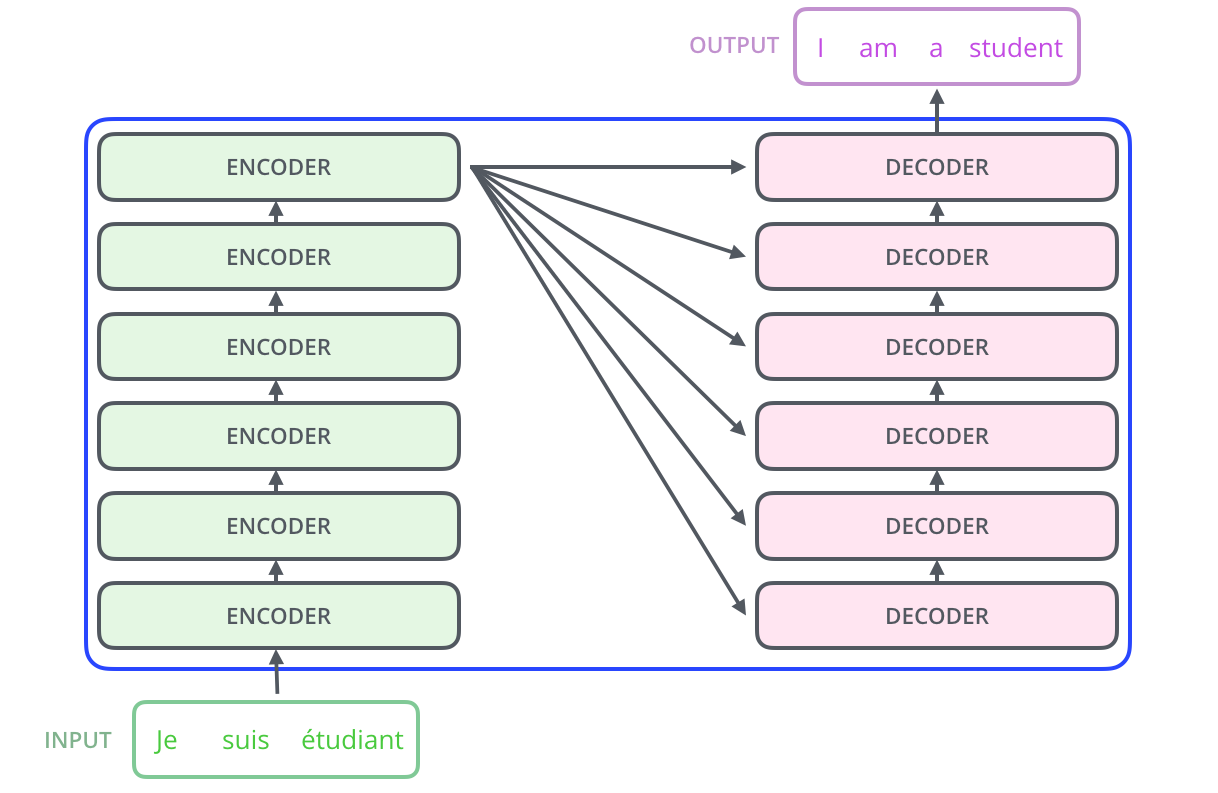
\includegraphics[scale=0.35]{images/The_transformer_encoder_decoder_stack}
        \caption{Encoder-decoder}
        \label{fig:encoder-decoder-stack}
    \end{center}
\end{figure}



\subsection{Encoder}
Các lớp của bộ mã hóa là độc lập nhau và có cấu trúc tương tự nhau. Đầu vào của lớp đầu tiên sẽ là các word embeddings đã được xử lý qua lớp positional encoding, các lớp phía trên sẽ có đầu vào là các vector output từ lớp ngay dưới. Các vector đầu vào của các lớp này được gọi là context vector.

Với mỗi lớp mã hóa sẽ bao gồm 2 lớp con:
\begin{itemize}
	\item Self-attetion: Với mỗi từ trong đoạn văn bản, xem xét độ liên quan của nó với các từ khác trong câu đầu vào. Đưa ra phân bố xác xuất đối với từng từ một.
	\item Feed forwarding: Mã hóa phân bố xác xuất tính toán được thành các context vector để đưa vào các lớp mã hóa phía trên.
\end{itemize}

\begin{figure}[H]
    \begin{center}
        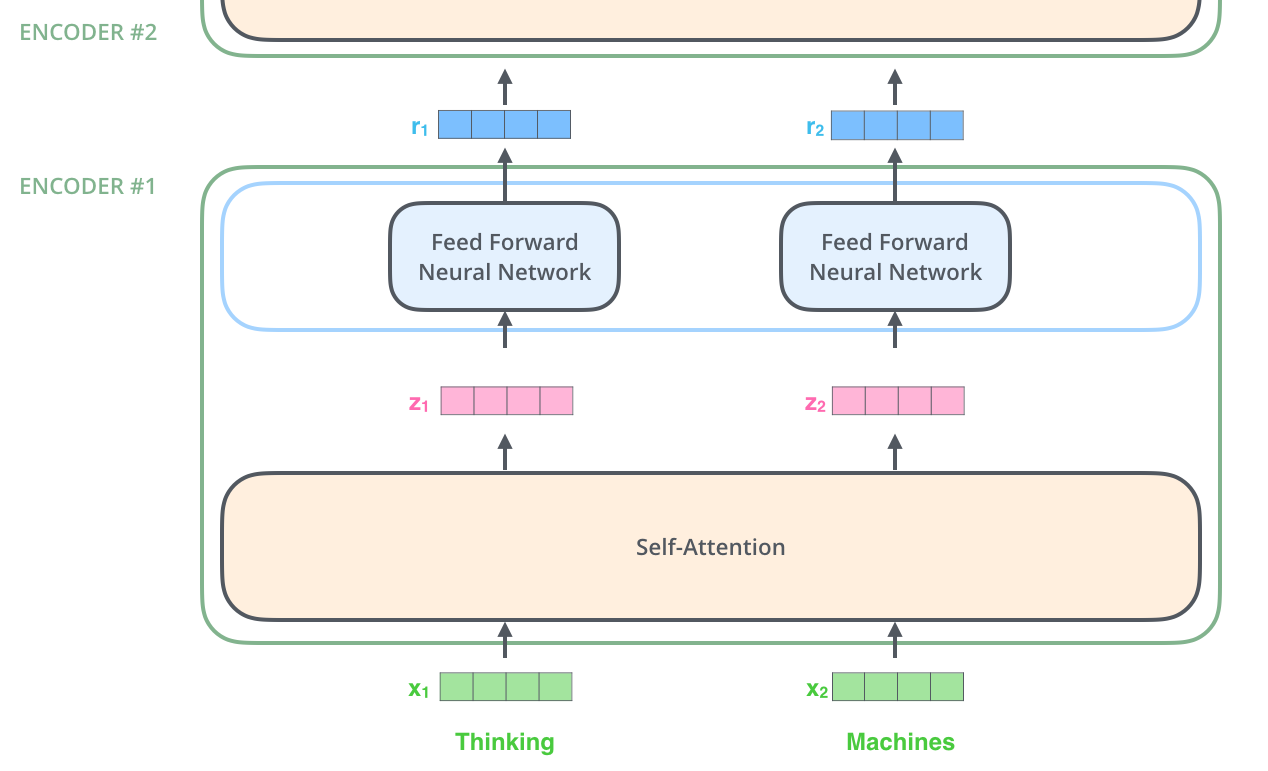
\includegraphics[scale=0.35]{images/encoder}
        \caption{Encoder}
        \label{fig:encoder}
    \end{center}
\end{figure}


\subsubsection{Cơ chế Self-attention}

Self-attention là một cơ chế mới được giới thiệu trong "attention is all need". Cơ chế này khác với cơ chế attention trong các mạng Seq2Seq trước đó. Self-attention cho phép ta biểu diễn lại mối quan hệ giữa các từ trong một đoạn văn bản.

\begin{figure}[H]
    \begin{center}
        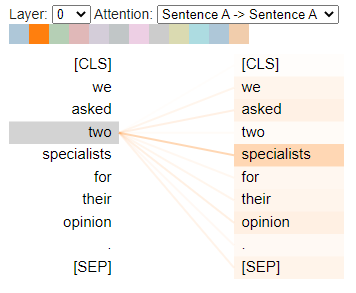
\includegraphics[scale=1.0]{images/self-attention}
        \caption{self-attention}
        \label{fig:self-attention}
    \end{center}
\end{figure}

Hình trên cho ta một minh họa về cơ chế self-attention. Xét từ "two", theo tư duy của con người, ta sẽ phân tích xem từ "two" trong câu đang có quan hệ gì với những từ khác. Ngoài ra, ta còn xem xét tầm quan trọng của các từ khác tác động lên ý nghĩa của câu. Từ đó mà ta có thể có được một cái nhìn rõ ràng hơn về vai trò của từ này trong câu.

Cụ thể hơn, khi mô hình xử lý từ "two", self-attention cho ta thấy được mối liên kết của nó với từ "specialists". Thể hiện vai trò của nó là dùng để chỉ số lượng của các chuyên gia là hai.

Việc tính toán ở mỗi lớp self attention được tính toán dựa trên công thức sau:

\begin{equation*}
	Attention = Softmax(\frac{QK^T}{\sqrt{d}})V
\end{equation*}

Trong đó, Q, K, V lần lượt là các ma trận Query, Key, Value. Hai ma trận query và key được dùng để tính toán mối quan hệ giữa các từ trong câu. Còn mỗi dòng thứ của ma trận V đại diện cho từ thứ i trong câu. Từ phân bố softmax, ta tính được context vector, tổng hợp được các thông tin của từ hiện tại và các từ liên quan đến nó. 

Trong công thức, ta thấy được tích vô hướng của ma trận Q và K được chuẩn hóa bởi hệ số $\sqrt{d}$ (d là số chiều của vector embedding). Lý do cho việc chuẩn hóa này là do khi d có giá trị lớn, tích vô hướng của Q và K sẽ có giá trị lớn theo do đó, nếu không chuẩn hóa về giá trị nhỏ hơn thì hàm softmax sẽ có độ hội tụ khá chậm

\begin{figure}[H]
    \begin{center}
        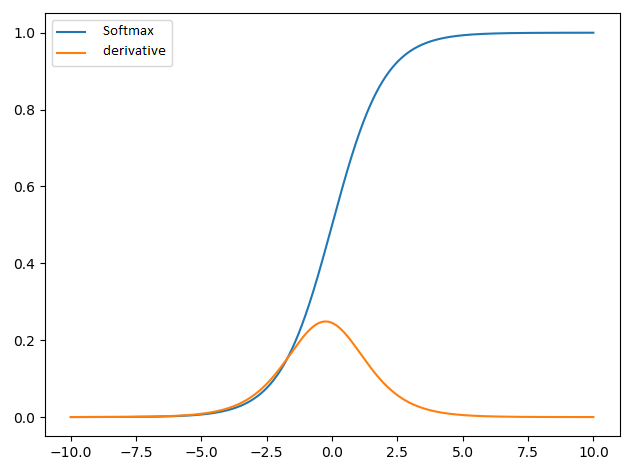
\includegraphics[scale=0.7]{images/softmax-func}
        \caption{Đồ thị hàm softmax và đạo hàm của một thành phần trong tập phân loại}
        \label{fig:softmax-func}
    \end{center}
\end{figure}


\begin{algorithm}[H]
    \caption{Self\_attention($context, w_K, w_Q, w_V$)}
    \begin{algorithmic}[1]
		\State \textbf{Result:} $Z$
		\State {$K \gets context \times w_K$}
		\State {$Q \gets context \times w_Q$}
		\State {$V \gets context \times w_V$}
		\State {$Score \gets QK^T$}
		\State {$Z \gets \frac{softmax(Score)}{\sqrt{d}}V$}
    \end{algorithmic}
\end{algorithm}

Từ công thức tính của self-attention, ta có thể thấy rõ sự khác biệt giữa bộ mã hóa của transformer và bộ mã hóa của các mô hình Seq2Seq sử dụng RNN. Đối với RNN, dữ liệu đầu vào phải được mã hóa một cách tuần tự. Trong khi đối với self-attention, các từ trong văn bản có thể được mã hóa một cái song song và không bị phụ thuộc vào nhau. Nhờ đó mà có thể tăng được hiệu quả tính toán.

\subsubsection{Cơ chế Multihead-attention}
Đầu ra của self-attention cho ta biết được mối quan hệ của các từ trong câu dựa trên một góc nhìn nào đó. Bằng các xếp chồng nhiều lớp self-attention lại với nhau. Ta có thể biết được sự liên quan của các từ ngữ trong câu với nhiều gốc nhìn khác nhau. Từ đó mà có được thông tin đầy đủ hơn về câu cần dịch. 

Cơ chế xếp chồng nhiều lớp self-attention lại với nhau được gọi là Multihead-attention. 

Ngoài ra, sử dụng cơ chế self-attention còn giúp ta tránh được trường hợp một từ phụ thuộc hoàn toàn vào chính nó. Ta mong muốn một phân bố xác suất quan hệ giữa một từ với các từ có ảnh hưởng đến nó.

Với việc sử dụng N lớp self-attention chạy song song với các bộ trọng số khác nhau, ta có được N ma trận context khác nhau. Lúc này, ta cần có một phương phát khác để tổng hợp thông tin từ các lớp self-attention này lại để đưa vào lớp feed-forward. 

\begin{figure}[H]
    \begin{center}
        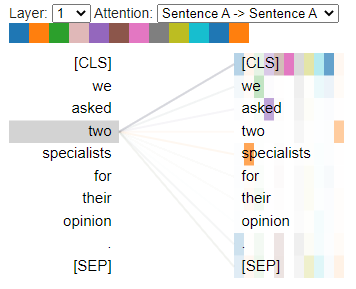
\includegraphics[scale=0.8]{images/multihead-context-vector}
        \caption{Multihead-context-vector}
        \label{fig:softmax-func}
    \end{center}
\end{figure}

Để làm được việc đó, transformer ghép theo chiều ngang các ma trận context lại rồi nhân với một bộ trọng số để đưa ra một kết quả duy nhất là một ma trận với các dùng là các context vector cũng đồng thời là đầu vào cho bộ giải mã ở phía trên.

\begin{figure}[H]
    \begin{center}
        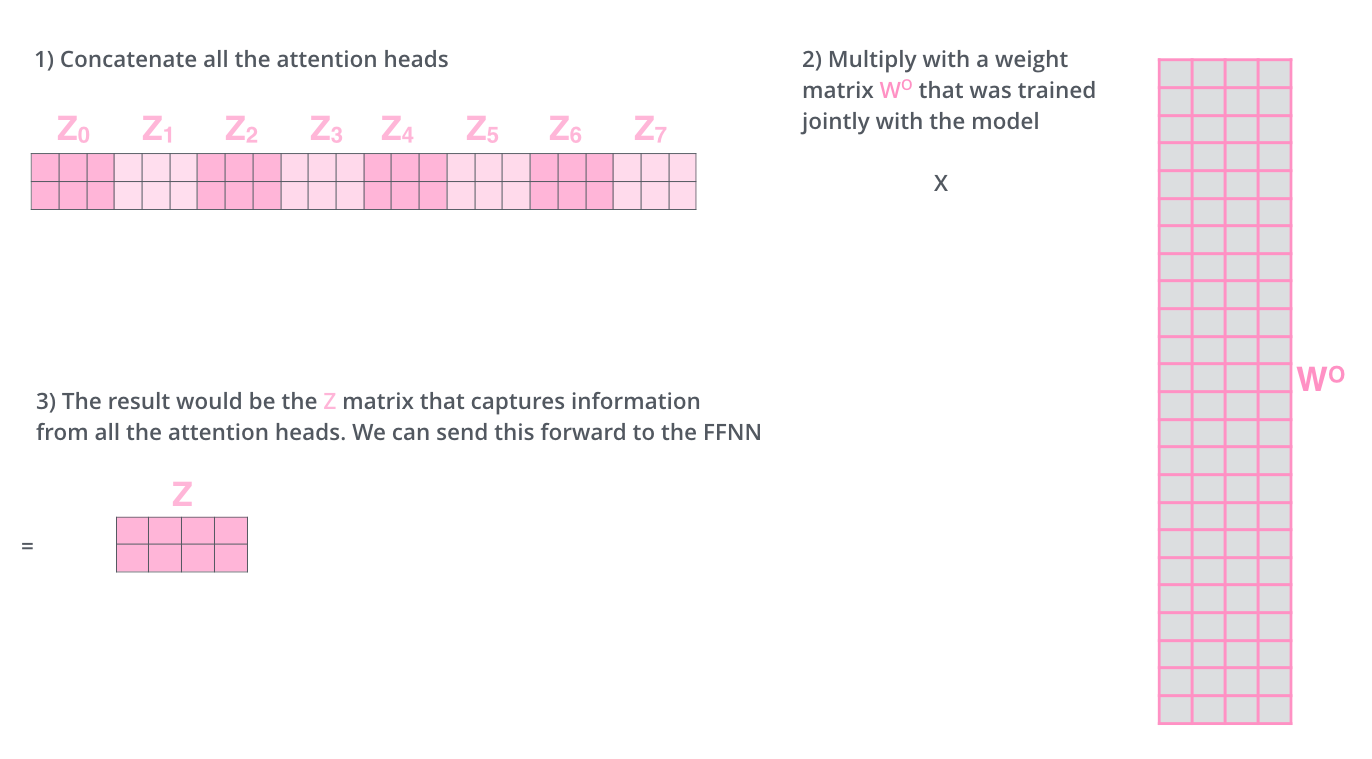
\includegraphics[scale=0.3]{images/transformer_attention_heads_weight_matrix_o}
        \caption{Multihead-context-vector}
        \label{fig:multihead-feed-forward}
    \end{center}
\end{figure}

Hình dưới minh họa cho việc sử dụng nhiều lớp self-attention trên cùng một câu với mỗi một màu tương ứng với kết quả của một lớp self-attention khác nhau.

\begin{algorithm}[H]
    \caption{Multihead attention($context$)}
    \begin{algorithmic}[1]
		\State \textbf{Result:} $Z \times w_O$
		\For{$1...number\_of\_head$}
			\State $Z_i \gets self\_attention(context, wK_i, wQ_i, wV_i)$
		\EndFor
		\State $Z \gets [Z_1, Z_2,... ,Z_{number\_of\_head}]$
    \end{algorithmic}
\end{algorithm}

\begin{figure}[H]
    \begin{center}
        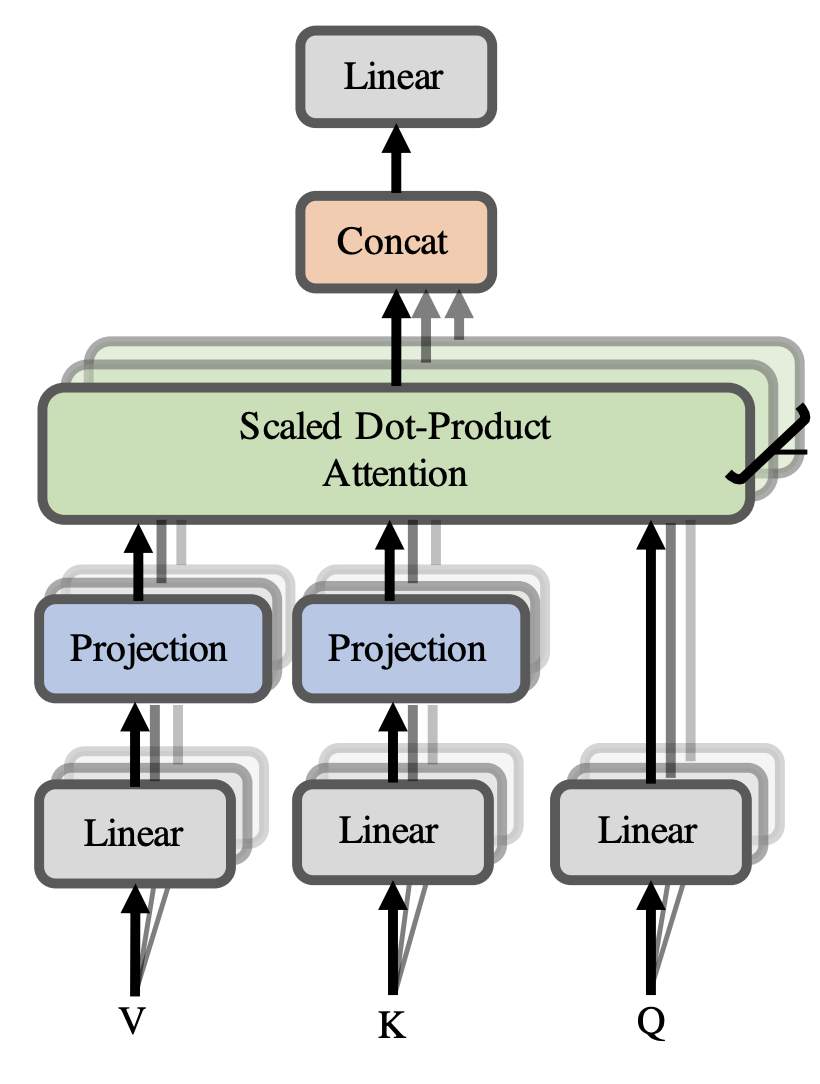
\includegraphics[scale=0.5]{images/multihead-attention}
        \caption{Multihead attention}
        \label{fig:multihead-attention}
    \end{center}
\end{figure}



\subsubsection{Positional encoding}

Cách tính toán song song của cơ chế self-attention dẫn đến một vấn đề đối với các từ trong đầu vào. Embeedings biểu diễn các từ này chưa biểu diễn được thông tin về thứ tự của các từ trong câu. Trong khi thông tin này là một thông tin quan trọng vì thay đổi vị trí của các từ có thể dẫn đến một câu hoàn toàn khác ý nghĩa.

Một ví dụ về việc đối chỗ một từ trong câu khiến cho ý nghĩa của câu trở nên trái ngược hoàn toàn:
\begin{itemize}
	\item "Please don't go! I love you!"
	\item "Please go! I don't love you!"
\end{itemize}

Transformer sử dụng cơ chế positional encoding. Cơ chế này giúp đưa thông tin về vị trí của các từ vào trong các embeddings. Cụ thể hơn, trước khi embeddings được đưa vào trong mô hình, nó được cộng với một vector tương ứng với vị trí trong câu. Những vector này tuân theo một một quy định nhất định. Chúng phải thể hiện được sự khác biệt về vị trí của các từ trong câu và cả khoảng cách của các từ trong câu. 

Công thức tính toán các vector này như sau: 
\begin{equation*}
	PE_{(pos, 2i)} = \sin{\frac{pos}{10000^{\frac{2i}{d_model}}}}
\end{equation*}
\begin{equation*}
	PE_{(pos, 2i+1)} = \cos{\frac{pos}{10000^{\frac{2i}{d_model}}}}
\end{equation*}

\begin{figure}[H]
    \begin{center}
        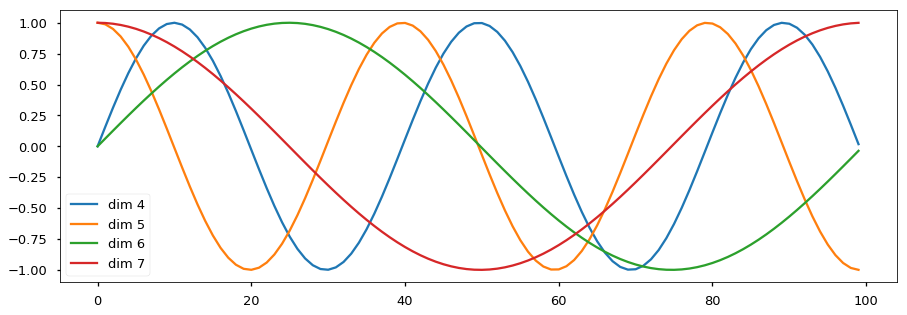
\includegraphics[scale=0.5]{images/positional-embedding}
        \caption{Đồ thị positional embedding}
        \label{fig:positional embedding}
    \end{center}
\end{figure}



\subsection{Decoder}
Các lớp của bộ giải mã cũng có 2 lớp con là Self-attention và Feed-forwarding giống với bộ mã hóa. Tuy nhiên giữa 2 lớp con này có một lớp trung gian là Encoder-Decoder attention. Lớp này có cơ chế giống với cơ chế attention trong mô hình Seq2Seq với thông tin của các hidden layer chính là đầu ra của bộ mã hóa.

\begin{figure}[H]
    \begin{center}
        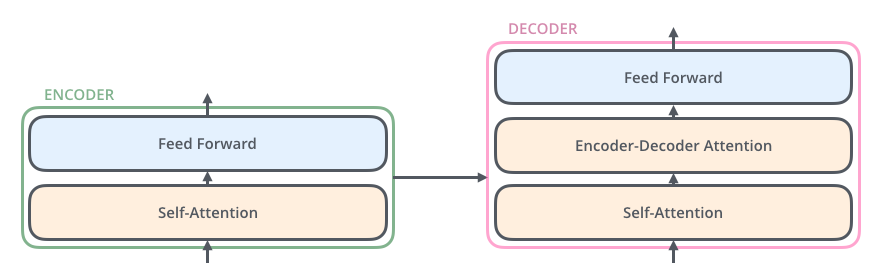
\includegraphics[scale=0.5]{images/Transformer_decoder}
        \caption{Transformer decoder}
        \label{fig:decoder}
    \end{center}
\end{figure}

\subsubsection{Masked self attention}

Khác với lớp self-attention ở bộ mã hóa, lớp masked self attention ở bộ giải mã chỉ tìm kiếm các mối quan hệ của từ hiện tại với các từ đã được giải mã trước đó. Do đó, trước khi thực hiện tính toán trên hàm softmax, giá trị score của các từ chưa được giải mã sẽ được gắn nhãn là $-\infty$. Sau đó, các bước tính toán sẽ tương tự như trong bộ mã hóa.

\begin{figure}[H]
    \begin{center}
        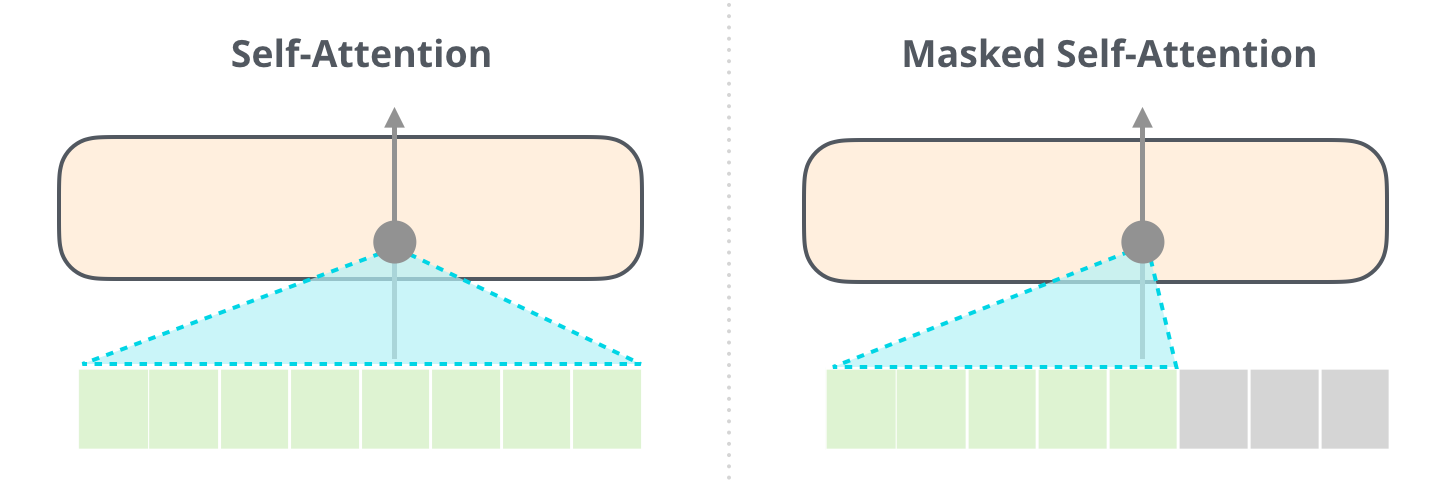
\includegraphics[scale=0.3]{images/self-attention-and-masked-self-attention}
        \caption{So sánh self attention và maked self attention}
        \label{fig:masked-self-attention}
    \end{center}
\end{figure}

Ta có thể điều chỉnh lại hàm self attention như sau:

\begin{algorithm}[H]
    \caption{Self\_attention($context, w_K, w_Q, w_V, masked$)}
    \begin{algorithmic}[1]
		\State \textbf{Result:} $Z$
		\State {$K \gets context \times w_K$}
		\State {$Q \gets context \times w_Q$}
		\State {$V \gets context \times w_V$}
		\State {$Score \gets QK^T$}
		\For{$i=masked + 1...len(context)$}
			\State Cột thứ i của $Score = -\infty$
		\EndFor
		\State {$Z \gets \frac{softmax(Score)}{\sqrt{d}}V$}
    \end{algorithmic}
\end{algorithm}

Tham số masked thể hiện kể từ vị trí này, các phần tử phía sau của score sẽ được gán giá trị $-\infty$. Hàm self\_attention được gọi bởi hàm multihead\_attention. Do đó, ta cần truyền thêm tham số masked vào hàm này. Ta mặc định masked = len(context), nhờ vậy mà mà cần truyền thêm tham số này khi gọi trong bộ mã hóa.


\subsubsection{encoder-decoder attention}
Một điểm khác biệt dễ thấy giữa bộ mã hóa và bộ giải mà là lớp encoder-decoder attention được đặt giữa 2 lớp self attetion lvâf feed-forward. Công dụng của lớp này giúp cho decoder có thể giải mã ra được các từ của văn bản đích dựa trên độ liên quan của mỗi từ với các từ trong văn bản nguồn. 

\begin{figure}[H]
    \begin{center}
        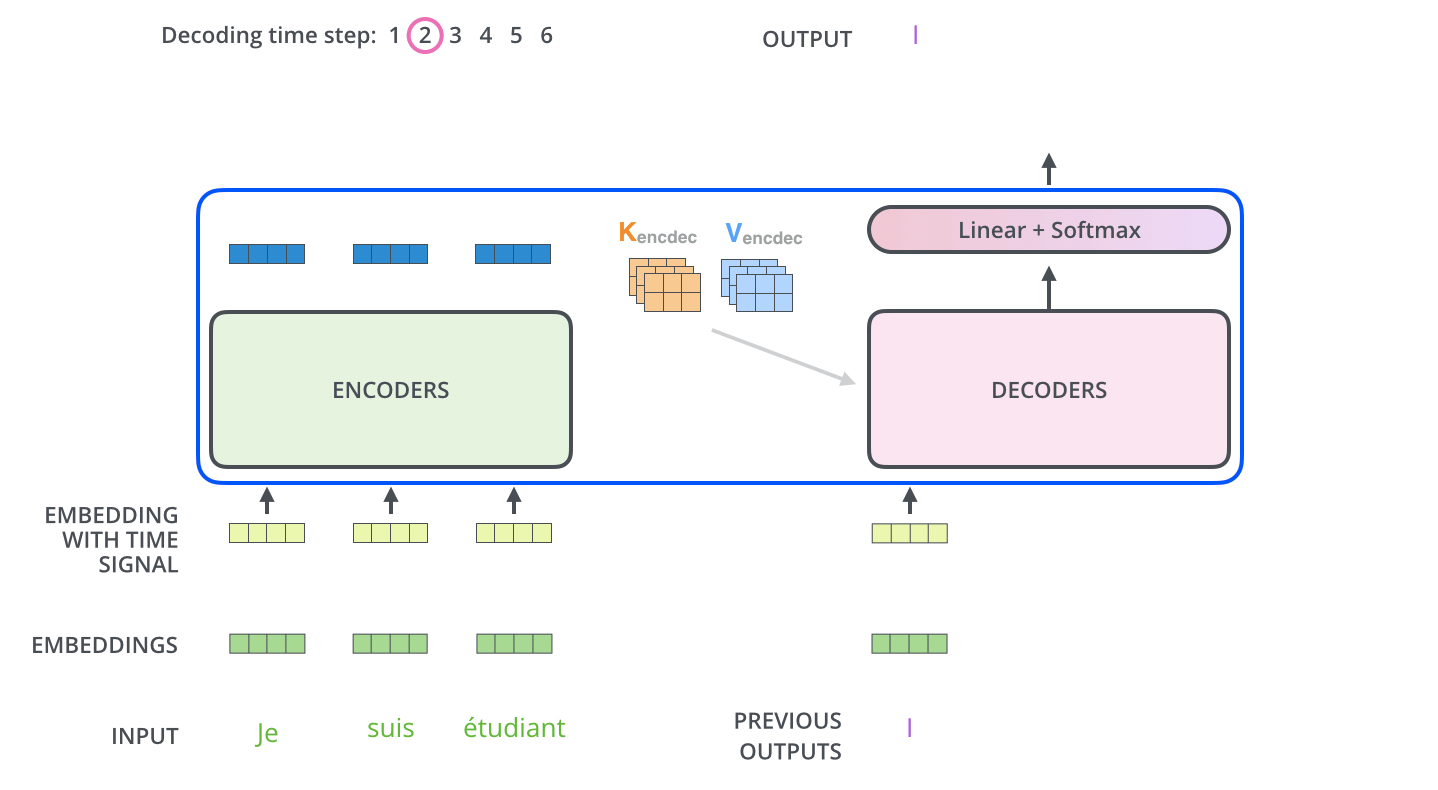
\includegraphics[scale=0.4]{images/encoder-decoder-attention}
        \caption{encoder-decoder-atention}
        \label{fig:encoder-decoder-attention}
    \end{center}
\end{figure}

Đầu ra lớp trên cùng của mã hóa sẽ được biến đổi thành 2 vector K và V. Quá trình giải mã được thực hiện như sau:


\begin{algorithm}[H]
    \caption{decoder(context, pos)}
    \begin{algorithmic}[1]
		\State \textbf{Result:} $feed\_forward(context)$
		\State $context \gets multihead\_attention(context, masked = pos)$
		\State $context \gets normalize(context)$
		\State $context \gets encoder\_decoder\_attention(K_{enc}, V_{env}, context)$
    \end{algorithmic}
\end{algorithm}

Để biểu thị cho mở đầu của đoạn văn bản và kết thúc của đoạn văn bản đến đánh dấu việc bắt đầu giải mã và kết thúc giải mã. Transformer sử dụng 2 token đặc biệt nằm tách biệt với bộ từ vựng: "<bos>" (begin of sentence) và "<eos>" (end of sentence).

Quá trình giải mã sẽ được bắt đầu với token "<bos>" và thực hiện một cách tuần từ cho đến khi giải mã ra token "<eos>". Từ được giải mã ở bước trước sẽ được sử dụng làm đầu vào cho bước giải mã tiếp theo. Cụ thể thuật toán của toàn bộ quá trình giải mã như sau:

\begin{algorithm}[H]
    \caption{Quá trình giải mã}
    \begin{algorithmic}[1]
		\State Khởi tạo $output_i \gets "<bos>"$
		\State Khởi tạo $i \gets 1$
		\Do
			\State $embed_i \gets position\_encoding(output_{i-1})$
			\State $context \gets embed_i$
			\For $j = 1...number\_decoder\_layer$
				\State $context \gets decoder(context, masked = i)$
			\EndFor
			\State $output_i \gets softmax(context)$
		\doWhile $output_i \neq "<eos>"$
    \end{algorithmic}
\end{algorithm}


\subsection{residuals}
Để tránh các trường hợp vanishing graident, Transformer kết hợp kiến trúc residual vào mạng encoder. Từ đó mà thông tin từ các lớp trước có thể được sử dụng lại trong khi huấn luyện các lớp sau.

với mỗi lớp con trong cả bộ mã hóa lẫn bộ giải mã, ta đặt thêm một lớp normalize vào ngay trên lớp con đó. Lớp normalize này nhận vào input là kết quả của lớp con ngay dưới của nó và cả đầu vào trước khi đi vào lớp con đó. Thưc hiện phép cộng 2 ma trận này và chuẩn hóa lại trước khi đưa vào lớp con phía trên.

\begin{figure}[H]
    \begin{center}
        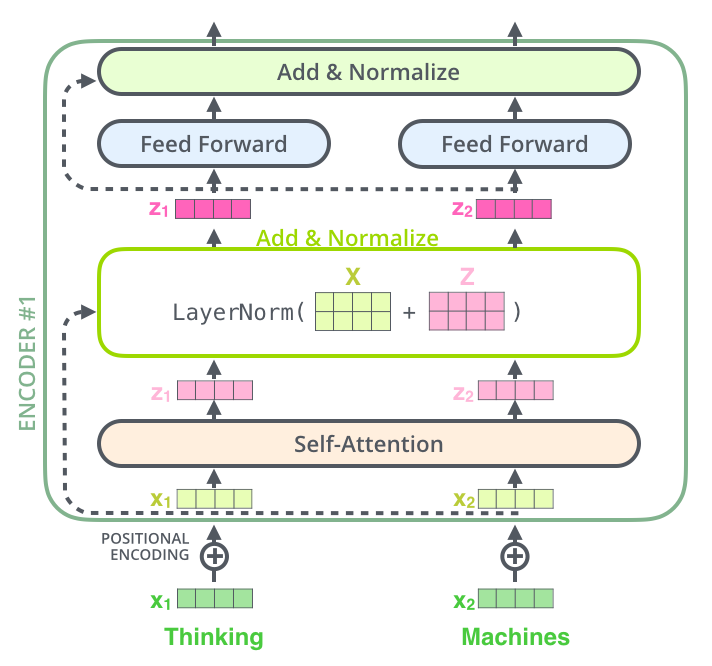
\includegraphics[scale=0.5]{images/residual}
        \caption{Residual}
        \label{fig:residual}
    \end{center}
\end{figure}


\subsection{Tổng kết mô hình}

Tổng kết lại, kiến trúc của Transformer bao gồm 2 thành phần chính là bộ mã hóa và bộ giải mã. Bộ mã hóa được tạo bởi nhiều lớp con gọi là các lớp mã hóa. Tương tự, bộ giải mã cũng được hình thành từ các lớp giải mã được xếp chồng lên nhau. Số lượng lớp con của bộ mã hóa bằng với số lượng lớp con của bộ giải mã.

Với mỗi lớp con của bộ mã hóa sẽ bao gồm một lớp multihead-attention và một lớp feed-forward. Ngoài ra còn áp dụng thêm kiến trúc residual block với các lớp normalize.

Với mỗi lớp giải mã, chúng được xếp chồng bởi 3 lớp con lần lượt là: masked-multihead-attention, encoder-decoder-attention và feed-forwarding. Lớp giải mã cũng được áp dụng kiến trúc residual block giúp mô hình tránh được hiện tượng vanishing gradient.

\begin{figure}[H]
    \begin{center}
        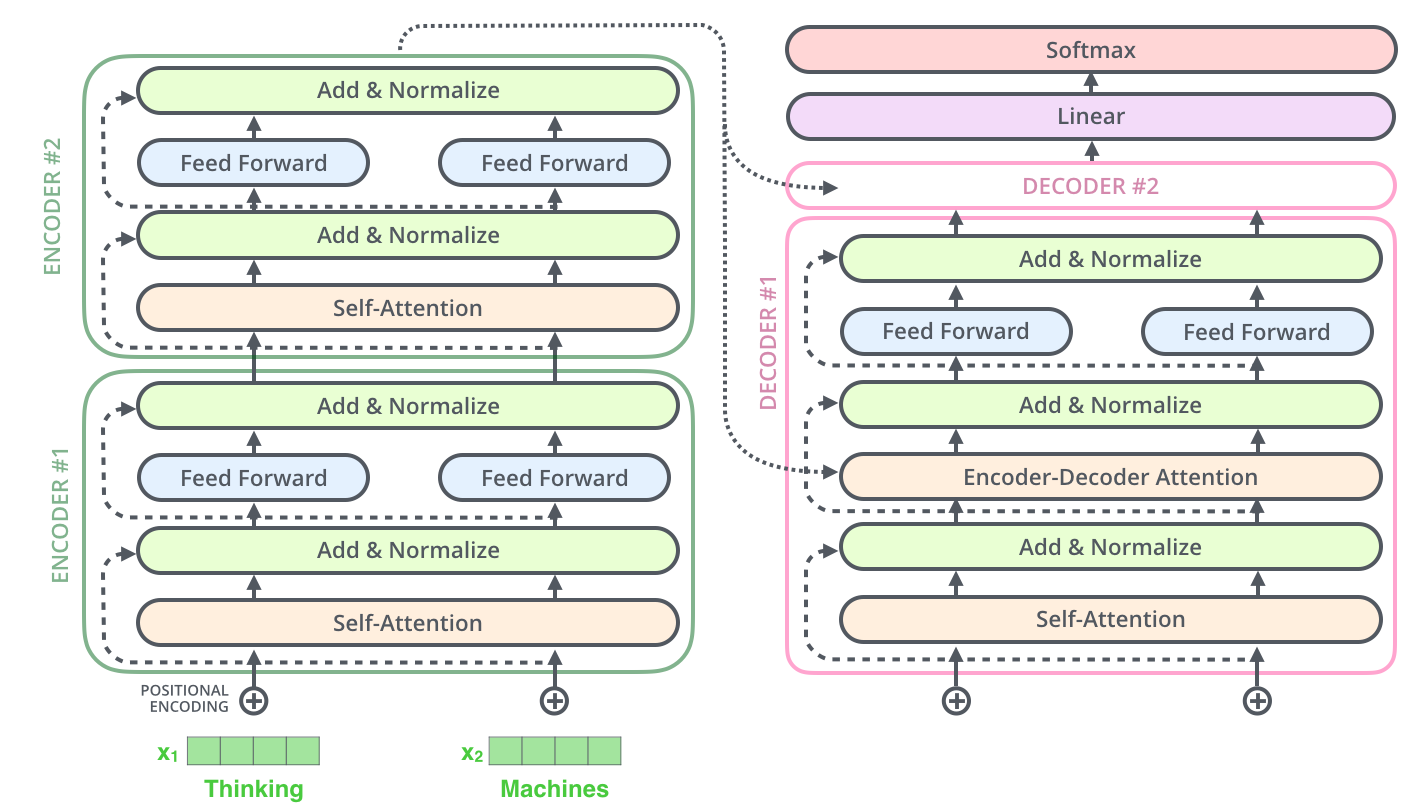
\includegraphics[scale=0.3]{images/transformer_sumary}
        \caption{Tổng kết mô hình transformer}
        \label{fig:transformer-summary}
    \end{center}
\end{figure}


\section{Mô hình WordGCN huấn luyện embedding cho bộ ngữ liệu}

\subsection{Lý thuyết đồ thị cơ bản}

\subsubsection{Định nghĩa đồ thị}

Đồ thị được định nghĩa là một cấu trúc rời rạc gồm các đỉnh và các cạnh nối các đỉnh đó. Ký hiệu biểu diễn một đồ thị như sau:
\begin{equation*}
	G = (V,E)
\end{equation*}

Trong đó, V là tập các đỉnh (Vertices) và E là tập các cạnh (Edges). Các cạnh trong tập E được bởi diễn bởi một cặp (x,y) với $x,y \in V$. Số lượng đỉnh của đồ thị là $|V| = n$, còn số lượng cạnh của đồ thị là $|E| = m$

\subsubsection{Các loại đồ thị}
Đơn đồ thị (simple graph) là đồ thị thỏa $\forall x,y \in V | $ không tồn tại quá 1 cạnh nối giữa hai đỉnh này.

Đa đồ thị (multigraph) là đồ thị thỏa $\forall x,y \in V | $ có thể có nhiều hơn 1 cạnh nối giữa 2 đỉnh này 

Giả đồ thị (speudo graph) là đồ thị chứa các đỉnh có khả năng nối cạnh với chính nó.

Đồ thị vô hướng (undirected graph) là đồ thị chứa các cạnh không định hướng. Nói cách khác, cạnh nối hai đỉnh x và y cũng sẽ được hiểu là cạnh đỉnh y với đỉnh x.

Đồ thị có hướng (directed graph) là đồ thị chứa các cạnh có hướng. nói cách khác, cạnh nói hai đỉnh x và y sẽ phân biệt với cạnh nối từ y đến x.

Đồ thị có trọng số là đồ thị mà các cạnh của đồ thị được biểu diễn bằng một trọng số nào đó. Lúc này mỗi cạnh $e \in E$ sẽ được biểu diễn bởi $(x, y, w)$. Với x và y là hai đỉnh của cạnh và w là trọng số của cạnh đó

Đồ thị không trọng số là đồ thị mà các cạnh của đồ thị không được biểu diễn bởi một trọng số.

(Ảnh minh họa các loại đồ thị)

Ngoài ra, khi kết hợp cách tính chất của các loại đồ thị khác nhau, ta có thể có được các dạng đồ thị khác như: Đơn đồ thị vô hướng, Đa đồ thị có hướng, Giả Đa đồ thị có hướng có trọng số,..

Đồ thị còn có thể phân loại theo đồ thị vô hạn và độ thị hữu hạn, chỉ số lượng cạnh và đỉnh của đồ thị là vô hạn hay có thể đếm được.

\subsubsection{vector đặc trưng (feature vectors)}

Lý thuyết đồ thị khi được áp dụng vào các bài toán học máy thường sẽ được bổ sung thêm khác khái niệm vector đặc trưng. Vector đặc trưng là những vector chỉ các đặc trưng của một đỉnh hoặc một cạnh của đồ thị. Các vector đặc trưng biểu diễn cho các đối tượng giống nhau phải có số lượng chiều như nhau.

Các vector này có thể có một cấu trúc đã được định nghĩa trước với tập các trường được khảo sát trên đối tượng tương ứng với đỉnh đang xét. Ngoài ra các vector của có thể được huấn luyện nhờ vào các mô hình học máy. Một bài toán được quan tâm đến khi nhắc đến các vector đặc trưng này là từ các liên kết của đồ thị và các context vector đã được định nghĩa trước, tìm ra các vector đặc trưng biểu diễn tốt cho các đối tượng đỉnh hoặc/và cạnh của đồ thị đó. Bài toán này được gọi là representation learning.

(Ảnh minh họa vector đặc trưng)

\subsubsection{Ma trận kề (adjacent matrix)}

Ma trận kề là ma trận chứa các thông tin về các cạnh nối giữa các đỉnh trong đồ thị. ma trận kề có kích thước $|V| \times |V|$. Phần tử ở hàng x cột y của ma trận chứa thông tin về kết nối giữa 2 đỉnh u và v và có giá trị như sau:
\begin{itemize}
	\item Đồ thị không trọng số: 0 hoặc x biểu thị hoặc không có cạnh nối giữa 2 điểm u và v hoặc có x cạnh đang nối giữa 2 đỉnh này.
	\item Đồ thị có trọng số: 0 hoặc w biểu thị hoặc không có cạnh nối giữa u và v hoặc có cạnh nối giữa u và v và trọng số của cạnh này là w
\end{itemize}

(Minh họa ma trận kề)

\subsubsection{Bậc của đồ thị}

Bậc của một đỉnh được định nghĩa là tổng số cạnh nối với đỉnh đó. Đối với đơn đồ thị, số cạnh nối với đỉnh đang xét cũng bằng số đỉnh kề với đỉnh đang xét. Bậc của đỉnh u được ký hiệu là deg(u).

Tính chất:
\begin{itemize}
	\item tổng số bậc của tất cả các đỉnh là số chẳn và có giá trị là $2m$ với m là số lượng cạnh của đồ thị
	\begin{equation*}
		\sum_{v \in V}{deg(v)} = 2m
	\end{equation*}
	\item Tổng số đỉnh có bậc lẻ là số chẵn.
	\item Đối với đồ thị vô hướng, tổng giá trị của hàng x hoặc cột x của ma trận kề biểu diễn đồ thị đó chính bằng deg(x)
\end{itemize}

Đối với đồ thị có hướng, bậc của một đỉnh còn được phân ra làm 2 thành phần:
\begin{itemize}
	\item Bán bậc vào là số lượng cạnh nối với đỉnh đang xét và có hường vào đỉnh đó. Ký hiệu bán bậc vào của đỉnh u là $deg^-(u)$
	\item Bán bậc ra là số lượng cạnh nối với đỉnh đang xét và có hường ra khỏi đỉnh đó. Ký hiệu bán bậc ra của đỉnh u là $deg^+(u)$
\end{itemize}

\begin{equation*}
	deg(u) = deg^-(u) + deg^+(u)
\end{equation*}

\subsection{Mô hình Graph Convolution Network và bài toán representation learning}

Để giải bài toán representation learning trên đồ thị, người ta đưa ra giả thuyết rằng, các nút trên đồ thị có khoảng cách càng gần nhau thì sẽ có các đặc tính giống nhau. Từ đó mà vector đặc trưng của những nút gần kế nhau cũng sẽ có khoảng cách gần nhau trong không gian latent.

(Hình minh họa representation learning)

Từ giả thuyết này, người ta đưa ra được ý tưởng chính của mạng GCN là sử dụng các vector đặc trưng của các nút kề với nút đang xét để học được đặc trưng của nút này.

Cho đồ thị $G = (V,E)$, có ma trận kề $A_{n \times n}$ và ma trận đặc trưng $X_{n \times d}$ với $n = |V|$ và d là chiều của ma trận đặc trưng. Mô hình GCN được kiến trúc bởi nhiều lớp ẩn chồng lên nhau. Gọi $H^{(l)}$ là đầu ra của lớp ẩn thứ l. $H^{(l)}$ là một ma trận có kích thức $n \times d_i$ với $d_i$ là số lượng đặc trưng của từng nút tại lớp l. Công thức tính $H^{(l)}$ được biểu diễn một cái đệ quy như sau:
\begin{equation*}
	H^{(l)} = 
	\begin{cases}
		f(H^{(l-1)}, A), & l > 0 \\
		X, & l = 0		
	\end{cases}
\end{equation*}

Trong đó, f là hàm tính đặc trưng của các nút dựa trên các lớp kề với nút đó. Do đó, f có biểu diễn như sau:
\begin{equation*}
	f(H^{(l)}, A) = \sigma(AH^{(l)}W^{(l)})
\end{equation*}

Với $W$ là ma trận chứa các tham số học có kích thước $d_l \times d_{l+1}$. Và $\sigma$ là hàm kích hoạt phi tuyến của mô hình. 

Với công thức của hàm f như trên, ta thấy được 2 phần thiếu sót như sau:
\begin{itemize}
	\item vector đặc trưng của nút u chỉ được tính bởi đặc trưng của các nút kề nó mà chưa được xét bởi các đặc trưng nội tại của nút u. Ta có thể giải quyết vấn đề này bằng các thêm các liên kết vòng (self connected edge) từ một nút đến chính nó. Ta định nghĩa ma trận $\tilde{A}$ là ma trận kề của G đã bổ sung các liên kết vòng:
	\begin{equation*}
		\tilde{A} = A + I
	\end{equation*} 
	\item Các đỉnh có bậc cao sẽ gây ảnh hưởng đến nhiều nút hơn các đỉnh khác. Và nó cũng sẽ được ảnh hưởng bởi nhiều đỉnh hơn các đỉnh khác. Theo như công thức f ở trên, các đỉnh có bậc cao sẽ ma giá trị rất lớn hoặc rất nhỏ dẫn đến việc cập nhập gradient chậm lại trong quá trình back-propagation. Để giải quyết vấn đề trên, GCN sử dụng phép chuẩn hóa Symetric normalized Laplacian để tránh sự thiên vị trong quá trình học.
	Từ đó mà ta có công thức đầy đủ của hàm f như sau:
	\begin{equation*}
		H^{(l+1)} = \sigma(\tilde{D}^{-1/2}\tilde{A}\tilde{D}^{1/2}H^{(l)}W^{(l)})
	\end{equation*}
\end{itemize}

Trong đó, $\tilde{D}$ là ma trận bậc của đồ thị G phép chuẩn hóa đối xứng laplacian có thể được hiểu là với mỗi $\tilde{A}_{u,v}$ sẽ được nhân với một lượng $\frac{1}{\sqrt{deg(u)}\sqrt{deg(v)}}$

\subsection{Mô hình WordGCN}

WordGCN là mô hình được ghép bởi 2 mô hình con là SynGCN và SemGCN. Cả hai mô hình trên đều áp dụng kiến trúc GCN để trích xuất các embeddings của các từ trong bộ ngữ liệu. Trong khi SynGCN trích xuất thông tin cú pháp (syntactic) của các từ thông qua các liên kết của chúng trong các đoạn văn bản. Thì SemGCN rút trích các đặc trưng về ngữ nghĩa (semantic) của các từ thông qua các mối quan hệ như: đồng nghĩa, trái nghĩa, từ viết tắt,...

\subsubsection{Mô hình SynGCN}

SynGCN quan tâm đến đặc trưng của một từ thông qua ví trị và vai trò của từ đó trong câu. theo universal dependency Mỗi từ trong câu sẽ có một mối quan hệ với một từ khác trong câu hoặc là chủ thể của cả câu (không có liên kết đến từ khác). Các mối quan hệ đó được gọi là các universal dependency. Từ đây, ta có thể xem mỗi câu $s = \{w_1, w_2,...,w_n\}$ trong bộ ngữ liệu là một đồ thị con dạng cây có hướng $G_s = (V_s, E_s)$ với các nút là các từ $V_s=\{w_1, w_2, w_3...,w_n\}$ và các dependency là các cạnh của đồ thị có dạng $(w_i, w_j, d_{ij})$ với $d_{ij}$ là mối quan hệ giữa $w_i$ và $w_j$. Lúc này, ta có thể áp dụng Thuật toán GCN lên đồ thị này. 

(Hình minh họa GCN)

Nhận xét thấy GCN áp dụng vào trường hợp này khá tương tự với mô hình CBOW. Mô hình này sử dụng tập các từ xung quanh $w_i$ để học các đặc trưng của $w_i$. Tập các từ như vậy được gọi là tập Context của $w_i$.

\begin{equation*}
	C_{w_i} = \{w_{i+j}: -c \leq j \leq c, j \neq 0\}
\end{equation*}

Trong đó, $c$ là kích thước của cửa sổ trượt.

Đối với SynGCN, tập Context của $w_i$ được định nghĩa là tập các các từ tương ứng với nút kề với $w_i$:
\begin{equation*}
	C_{w_i} = N(w_i) = \{w_j: (w_i, w_j, l_{i,j}) \in E_s\}
\end{equation*}


\subsubsection{Mô hình SemGCN}

Các embedding sau khi được huấn luyện qua mạng SynGCN sẽ được đưa vào mạng SemGCN để học các đặc trưng về ngữ nghĩa (semantic context). Mô hình cho phép học các mối quan hệ có tính đối xứng lẫn các mối quan hệ không đối xứng. Đối với các mô hình trước đây, hoặc là chúng chỉ có thể giải quyết các mối quan hệ đối xứng hoặc chưa xử lý tốt vối các môi không đối xứng. Gọi G =(V,E) là đồ thị được tạo thành từ các ngữ nghĩa trong bộ dữ liệu. Ta sẽ có các đỉnh là các từ trong bộ nghữ liệu còn các cạnh là các mối quan hệ giữa chúng. Các cạnh trong G có định hướng. Đối với 2 từ x và y có liên kết đối xứng thì giữa 2 đỉnh tương ứng với x và y sẽ có 2 cạnh ngược hướng.

(Hình minh họa SemGCN)

Sau khi có được đồ thì biểu diễn, ta có thể sử dụng thuật toán GCN để tối ưu các embeddings đã được huấn luyện từ mô hình SynGCN.